% ------------------------------------------------------------------------------
% TYPO3 CMS 8.3 - What's New - Chapter "Introduction" (English Version)
%
% @author	Michael Schams <schams.net>
% @license	Creative Commons BY-NC-SA 3.0
% @link		http://typo3.org/download/release-notes/whats-new/
% @language	English
% ------------------------------------------------------------------------------
% LTXE-CHAPTER-UID:		7fdf26cc-362160ab-d6c8b905-19722b20
% LTXE-CHAPTER-NAME:	Introduction
% ------------------------------------------------------------------------------

\section{Inleiding}
\begin{frame}[fragile]
	\frametitle{Inleiding}

	\begin{center}\huge{Inleiding}\end{center}
	\begin{center}\huge{\color{typo3darkgrey}\textbf{De feiten}}\end{center}

\end{frame}

% ------------------------------------------------------------------------------
% LTXE-SLIDE-START
% LTXE-SLIDE-UID:		f40ffea9-13455165-3b4af5c5-c336bfa6
% LTXE-SLIDE-ORIGIN:	ca3596df-e5f14953-556d9c5f-a8a689fe English
% LTXE-SLIDE-TITLE:		TYPO3 CMS 8.2 and 8.3 - The Facts
% ------------------------------------------------------------------------------
\begin{frame}[fragile]
	\frametitle{Inleiding}
	\framesubtitle{TYPO3 CMS 8.2 en 8.3 - De feiten}

	\textbf{TYPO3 CMS 8.2}
	\begin{itemize}
		\item Publicatiedatum: 5 juli 2016
		\item Publicatietype: Sprint Release
		\item Slogan: Upgrades
	\end{itemize}

	\vspace{0.6cm}

	\textbf{TYPO3 CMS 8.3}
	\begin{itemize}
		\item Publicatiedatum: 30 augustus 2016
		\item Publicatietype: Sprint Release
		\item Slogan: Bewerken in Frontend powereditie
	\end{itemize}

%	\begin{figure}
%		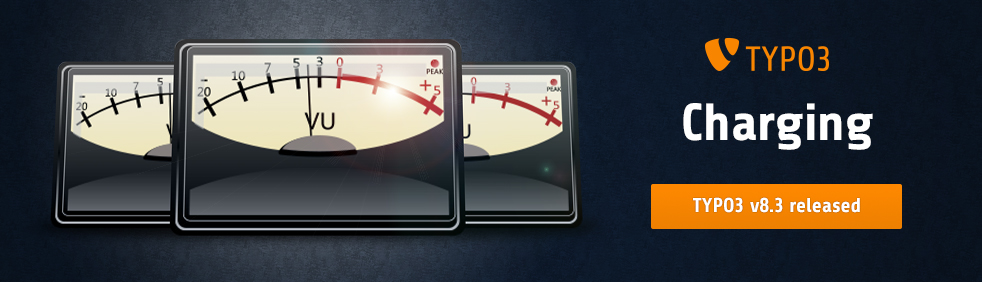
\includegraphics[width=0.95\linewidth]{Introduction/typo3cms83-banner.jpg}
%	\end{figure}

\end{frame}

% ------------------------------------------------------------------------------
% LTXE-SLIDE-START
% LTXE-SLIDE-UID:		a3e603b4-a2b7bd35-2aaa086e-44159ec5
% LTXE-SLIDE-ORIGIN:	1be10378-6e990dd6-2cca609a-c778c43c English
% LTXE-SLIDE-TITLE:		System Requirements
% ------------------------------------------------------------------------------
\begin{frame}[fragile]
	\frametitle{Inleiding}
	\framesubtitle{Systeemeisen}

	\begin{itemize}
		\item PHP:\tabto{2.2cm}versie 7
		\item MySQL:\tabto{2.2cm}versie 5.5 tot 5.7
		\item Schijfruimte:\tabto{2.2cm}min 200 MB
		\item PHP instellingen:

			\begin{itemize}
				\item \texttt{memory\_limit} >= 128M
				\item \texttt{max\_execution\_time} >= 240s
				\item \texttt{max\_input\_vars} >= 1500
				\item compilation option \texttt{-}\texttt{-disable-ipv6} moet \underline{niet} worden gebruikt
			\end{itemize}

		\item De backend vereist Microsoft Internet Explorer 11 of nieuwer,
			Microsoft Edge, Google Chrome, Firefox, Safari of een andere moderne
			compatibele browser

	\end{itemize}

\end{frame}

% ------------------------------------------------------------------------------
% LTXE-SLIDE-START
% LTXE-SLIDE-UID:		b5d80aed-b80f6d53-dba6bd4f-3574c69b
% LTXE-SLIDE-ORIGIN:	ed8e8933-d90001c7-f7548bd3-80e549cb English
% LTXE-SLIDE-TITLE:		Development And Release Timeline
% ------------------------------------------------------------------------------
\begin{frame}[fragile]
	\frametitle{Inleiding}
	\framesubtitle{Planning voor ontwikkeling en publicatie}

	\begin{figure}
		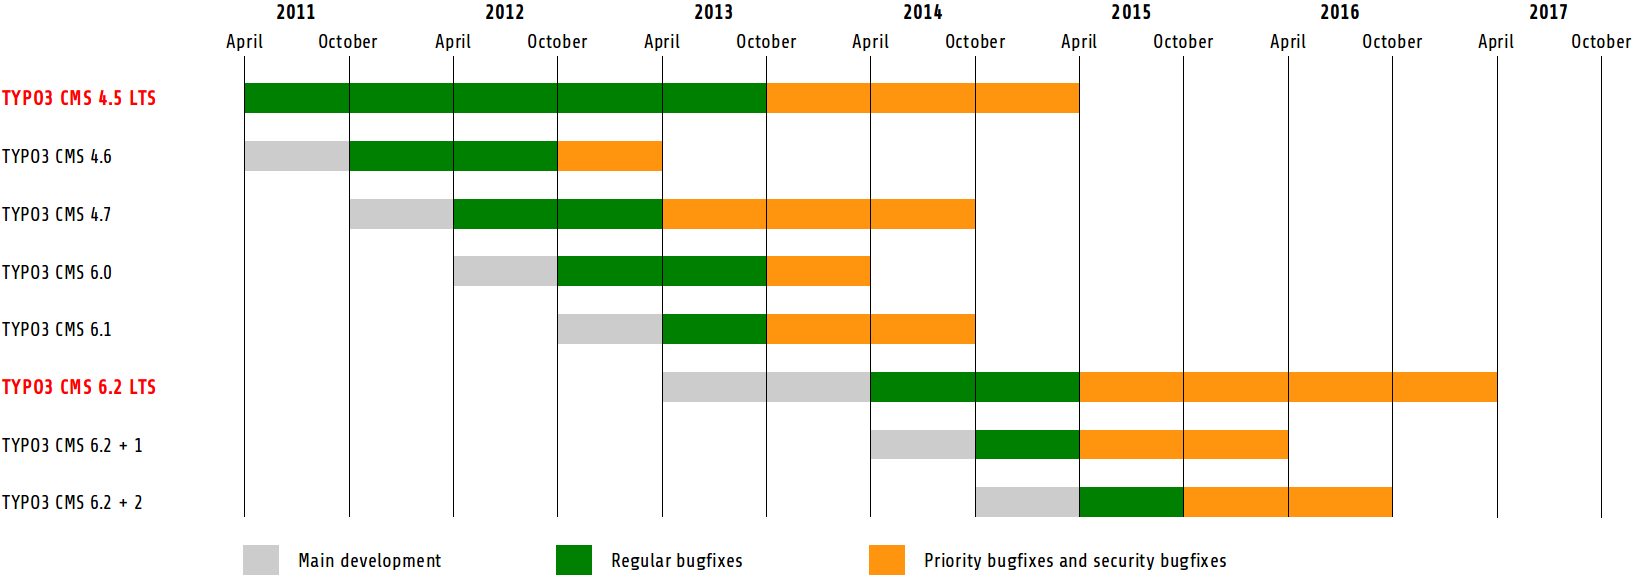
\includegraphics[width=1\linewidth]{Introduction/ReleaseAgenda.png}
	\end{figure}

\end{frame}

% ------------------------------------------------------------------------------
% LTXE-SLIDE-START
% LTXE-SLIDE-UID:		1d7e8539-92a15834-db5f4d19-fa3df865
% LTXE-SLIDE-ORIGIN:	01225efb-e9fdbaff-726e5fed-5b7f0003 English
% LTXE-SLIDE-TITLE:		TYPO3 CMS Roadmap
% ------------------------------------------------------------------------------
\begin{frame}[fragile]
	\frametitle{Inleiding}
	\framesubtitle{TYPO3 CMS Roadmap}

	Publicatiedatums en primaire focus:

	\begin{itemize}

		\item v8.0 \tabto{1.1cm}22 mrt 2016\tabto{3.4cm}Last minute toevoegingen
		\item v8.1 \tabto{1.1cm}03 mei 2016\tabto{3.4cm}Cloud-integratie
		\item
			\begingroup
				\color{typo3orange}
					v8.2 \tabto{1.1cm}05 jul 2016\tabto{3.4cm}Upgrades
			\endgroup
		\item
			\begingroup
				\color{typo3orange}
					v8.3 \tabto{1.1cm}30 aug 2016\tabto{3.4cm}Bewerken in Frontend powereditie
			\endgroup
		\item v8.4 \tabto{1.1cm}18 okt 2016\tabto{3.4cm}\textit{onbekend}
		\item v8.5 \tabto{1.1cm}20 dec 2016\tabto{3.4cm}Integrator-ondersteuning
		\item v8.6 \tabto{1.1cm}14 feb 2017\tabto{3.4cm}\textit{onbekend}
		\item v8.7 \tabto{1.1cm}04 apr 2017\tabto{3.4cm}LTS Voorbereiding

	\end{itemize}

	\smaller
		\url{https://typo3.org/typo3-cms/roadmap/}\newline
		\url{https://typo3.org/news/article/kicking-off-typo3-v8-development/}
	\normalsize

\end{frame}

% ------------------------------------------------------------------------------
% LTXE-SLIDE-START
% LTXE-SLIDE-UID:		3c5b30f7-4912b401-ac42e3f9-f3c23532
% LTXE-SLIDE-ORIGIN:	793cc944-52bccf17-ba7c4c9c-661e8993 English
% LTXE-SLIDE-TITLE:		Installation
% ------------------------------------------------------------------------------
\begin{frame}[fragile]
	\frametitle{Inleiding}
	\framesubtitle{Installatie}

	\begin{itemize}
		\item Officiële installatieprocedure op Linux/Mac OS X\newline
			(DocumentRoot bijvoorbeeld \texttt{/var/www/site/htdocs}):
		\begin{lstlisting}
			$ cd /var/www/site
			$ wget --content-disposition get.typo3.org/8.3
			$ tar xzf typo3_src-8.3.0.tar.gz
			$ cd htdocs
			$ ln -s ../typo3_src-8.3.0 typo3_src
			$ ln -s typo3_src/index.php
			$ ln -s typo3_src/typo3
			$ touch FIRST_INSTALL
		\end{lstlisting}

		\item Symbolische links op Microsoft Windows:

			\begin{itemize}
				\item Gebruik \texttt{junction} op Windows XP/2000
				\item Gebruik \texttt{mklink} op Windows Vista en Windows 7
			\end{itemize}

	\end{itemize}
\end{frame}

% ------------------------------------------------------------------------------
% LTXE-SLIDE-START
% LTXE-SLIDE-UID:		af17efdf-fd3a8353-bbe3ff10-964e8c05
% LTXE-SLIDE-ORIGIN:	4c0c3586-154241f9-4c859652-03bcc92e English
% LTXE-SLIDE-TITLE:		Upgrade to TYPO3 CMS 7
% ------------------------------------------------------------------------------
\begin{frame}[fragile]
	\frametitle{Inleiding}
	\framesubtitle{Upgrade naar TYPO3 CMS 8.x}

	\begin{itemize}
		\item Upgrades alleen mogelijk vanaf TYPO3 CMS 7.6 LTS
		\item TYPO3 CMS < 7.6 LTS moet eerst naar TYPO3 CMS 7.6 LTS bijgewerkt worden
	\end{itemize}

	\begin{itemize}

		\item Upgrade-instructies:\newline
			\smaller\url{http://wiki.typo3.org/Upgrade#Upgrading_to_8.3}\normalsize
		\item Officiële TYPO3-handleiding "TYPO3 Installation and Upgrading":
			\smaller\url{http://docs.typo3.org/typo3cms/InstallationGuide}\normalsize
		\item Algemene aanpak:
			\begin{itemize}
				\item Controleer minimale systeemeisen \small(PHP, MySQL, etc.)
				\item Bekijk \textbf{deprecation\_*.log} in oude TYPO3 installatie
				\item Update alle extensies naar laatste versie
				\item Zet nieuwe broncode neer en start Install Tool -> Upgrade Wizard
				\item Bekijk startmodule voor backend gebruikers (optioneel)
			\end{itemize}
	\end{itemize}

\end{frame}

% ------------------------------------------------------------------------------

% ------------------------------------------------------------------------------
% LTXE-SLIDE-START
% LTXE-SLIDE-UID:		ea530ff8-06fd6424-f1c460b7-10591652
% LTXE-SLIDE-ORIGIN:	36c478bf-991c3c9c-1b55ed59-ee1ad72e English
% LTXE-SLIDE-TITLE:		PHP Version 7
% ------------------------------------------------------------------------------
\begin{frame}[fragile]
	\frametitle{Inleiding}
	\framesubtitle{PHP Version 7}

	\begin{itemize}

		\item PHP 7.0 is de minimale eis voor TYPO3 CMS 8.x
		\item TYPO3 zal volgende PHP 7 versies ondersteunen wanneer deze uitkomen
		\item Deze versie geeft significant meer prestaties op het hele systeem

		\item Niet alleen backendgebruikers merken een soepelere interface, maar ook het
			nieuwe record voor een volledig gecachete pagina in de frontend is nu minder
			dan 7 milliseconden, wat ongeveer 40\% sneller is in vergelijking met dezelfde
			website met PHP versie 5.5

		\item We zijn ook begonnen nieuwe features van deze PHP-versie te gebruiken, bijvoorbeeld
			de cryptografisch veilige pseudo-random generatoren worden al ingezet

	\end{itemize}

\end{frame}

% ------------------------------------------------------------------------------
